\documentclass[UTF8,a4paper,11pt]{ctexart}

\usepackage[margin=2.3cm]{geometry}
\usepackage{graphicx}
\usepackage{amsmath,amssymb}
\usepackage{booktabs}
\usepackage{hyperref}
\usepackage{caption}
\usepackage{subcaption}
\usepackage{enumitem}
\usepackage{xcolor}

\hypersetup{
  colorlinks=true,
  linkcolor=blue,
  citecolor=blue,
  urlcolor=blue
}

\graphicspath{{../figures/}}

\title{\bfseries 双栅 WSe$_2$ 复数二次谐波场零点与相位绕转的数值认证\\
\large Gate-programmable zeros and phase winding of the scalar complex SHG field in exciton-polaron-mediated bilayer WSe$_2$}
\author{}
\date{}

\begin{document}
\maketitle

\section*{摘要}
本文围绕 Cha 等人在双栅双层 WSe$_2$ 中通过 layer-dependent exciton-polaron effect 增强共振二次谐波产生的工作，进一步细化一个新的可验证创新点：双栅调控 exciton-polaron 共振，实现双层 WSe$_2$ 标量复 SHG 场的电控零点与相位绕转。本文不把普通 SHG 强度增强作为创新本身，而是把研究对象从强度调制推进到复数二次谐波场 $E_{2\omega}$ 的实部、虚部、相位和零点结构。

我们构建了一个 literature-constrained phenomenological Python 模型：先将顶栅和底栅电压映射到载流子密度 $n$ 与位移场 $D$，再用层分辨复 Lorentz 振子描述 neutral exciton 与 exciton-polaron 通道，最后通过 2H 双层的相干场求和得到标量复 SHG 场。模型数值认证了在合理参数范围内，复 SHG 场可以被门压推近相消零点，并在围绕零点的 gate loop 上产生相位绕转。相位分辨 heterodyne SHG 可作为实验验证路径。

\paragraph{English central claim.}
We propose and numerically validate a gate-programmable scalar complex-SHG-field zero in exciton-polaron-mediated bilayer WSe$_2$. The central advance is not stronger SHG intensity, but electrical control of the phase and topology of the emitted second-harmonic field.

\section{主论文基线与创新边界}
主论文基线是 Cha et al. 2024 的 dual-gated bilayer WSe$_2$ resonant SHG 工作~\cite{cha2024}。该论文的关键事实是：双栅结构可以使空穴在双层中产生层选择性分布，使某一层进入 exciton-polaron 态，而另一层更接近 neutral-exciton 响应。由于上下层的共振条件和非线性响应不再等价，原本接近反演对称抵消的 2H 双层可以产生显著的 resonant SHG 增强或淬灭。

因此，本文不能把 dual-gated bilayer WSe$_2$、layer-dependent exciton-polaron、低场 SHG 增强或普通 SHG 开关写成自己的创新。这些是基线工作已经建立的实验平台和强度响应。本文的创新边界是：在同一类双栅 exciton-polaron 平台上，不再只研究 SHG intensity，而是研究复数 SHG 场 $E_{2\omega}$ 本身是否可以通过门压主动推过相干零点，并由此产生相位跳变和绕转。

\section{文献缺口：从强度控制到复场控制}
电控 SHG 强度并不是空白问题。Seyler 等人在 monolayer WSe$_2$ transistor 中已经展示了电掺杂对二阶非线性响应的调控，低温下 A-exciton 附近 SHG 强度可调超过一个数量级，室温下也接近四倍~\cite{seyler2015}。这说明“电控 SHG 强度”本身不足以构成本文的核心创新。

另一方面，SHG 场具有复相位并可发生层间相干干涉也已有先例。Kim 等人的 Second-Harmonic Young Interference 工作用 spectral phase interferometry 证明了 atom-thin heterocrystals 中两层发出的二次谐波场会相干干涉，并可解析材料相关的 SH phase delay~\cite{kim2020}。这说明复数二阶非线性极化率和 SHG 相位并不是形式上的数学量，而是可以实验访问的物理量。

真正的缺口是：已有工作要么关注电控强度，要么关注静态材料组合或扭角导致的 SHG 相位干涉。仍然缺少一种以双栅为主动控制参数、以 exciton-polaron 共振为相位旋转源、以复 SHG 场零点和相位绕转为核心判据的机制方案。本文正是在这个缺口上提出并数值认证一个单一创新点。

\section{核心物理命题}
本文的核心命题可以写成一句话：双栅调控 exciton-polaron 共振，实现双层 WSe$_2$ 标量复 SHG 场的电控零点与相位绕转。这里的“标量复 SHG 场”指固定入射和探测偏振通道下的 $E_{2\omega}$ 复振幅，而不是完整 Jones vector 偏振态。这样做的好处是主线集中、实验判据清晰，也避免把本文扩展成 polarization singularity 的主张。

在 2H bilayer WSe$_2$ 中，上下两层二阶响应近似反号。若门压使上层和下层的复数非线性极化率分别为 $\chi_{\mathrm{top}}^{(2)}$ 和 $\chi_{\mathrm{bottom}}^{(2)}$，则最小模型中的发射场可以写成
\begin{equation}
  E_{2\omega} = \chi_{\mathrm{top}}^{(2)}-\chi_{\mathrm{bottom}}^{(2)} .
\end{equation}
普通强度实验只看 $|E_{2\omega}|^2$，而相位分辨实验可以恢复 $\arg(E_{2\omega})$ 以及 $\mathrm{Re}(E_{2\omega})$、$\mathrm{Im}(E_{2\omega})$。当
\begin{equation}
  \mathrm{Re}(E_{2\omega})=0,\qquad \mathrm{Im}(E_{2\omega})=0
\end{equation}
在二维门压参数空间中同时成立时，就形成一个标量复场零点。

双栅参数空间提供两个独立控制量，通常可重写为 carrier density $n$ 和 displacement field $D$。复场零点需要满足两个方程，因此在二维参数空间中出现孤立零点是自然的。围绕该零点走闭合 gate loop $\mathcal{C}$ 时，定义绕数
\begin{equation}
  W = \frac{1}{2\pi}\oint_{\mathcal{C}} d\,\arg E_{2\omega}.
\end{equation}
若路径围绕复场零点，$W$ 可以接近整数。这正是本文把强度调制升级为复场拓扑响应的关键。

\section{可复现 Python 模型}
Python 模型采用定性到半定量之间的 literature-constrained phenomenological 形式。它不拟合 Cha 2024 原始实验数据，也不试图替代第一性原理或电磁场仿真。模型的目标是数值认证机制链条是否自洽：gate 改变层分辨载流子分布，载流子分布改变 neutral-exciton 与 exciton-polaron 的复 Lorentz 响应，层分辨复响应相干叠加后产生接近零点的标量复 SHG 场。

模型分为五个模块。第一，gate coordinate 模块将 $V_t$、$V_b$ 映射为归一化 $n$ 和 $D$。第二，susceptibility 模块为每一层构造 neutral-exciton 与 exciton-polaron 两个复 Lorentz 振子，并允许门压导致振子强度、线宽和共振位置变化。第三，SHG field 模块实现 $E_{2\omega}=\chi_{\mathrm{top}}^{(2)}-\chi_{\mathrm{bottom}}^{(2)}$ 的 2H 双层相干场求和。第四，topology 模块寻找近零点并计算闭合路径相位绕数。第五，heterodyne 模块模拟样品 SHG 与参考 SHG 的干涉条纹。

为避免漂亮但不可测的数值结果，模型加入轻量实验可实现约束：门压和位移场保持在归一化合理范围内，路径上除接近零点的区域外保持可检测相对强度，线宽和振子强度的扫描避免极端值。本文不做完整 device optimizer，而是用这些 filter 排除明显不合理的参数选择。

\section{数值认证结果}
\begin{figure}[htbp]
  \centering
  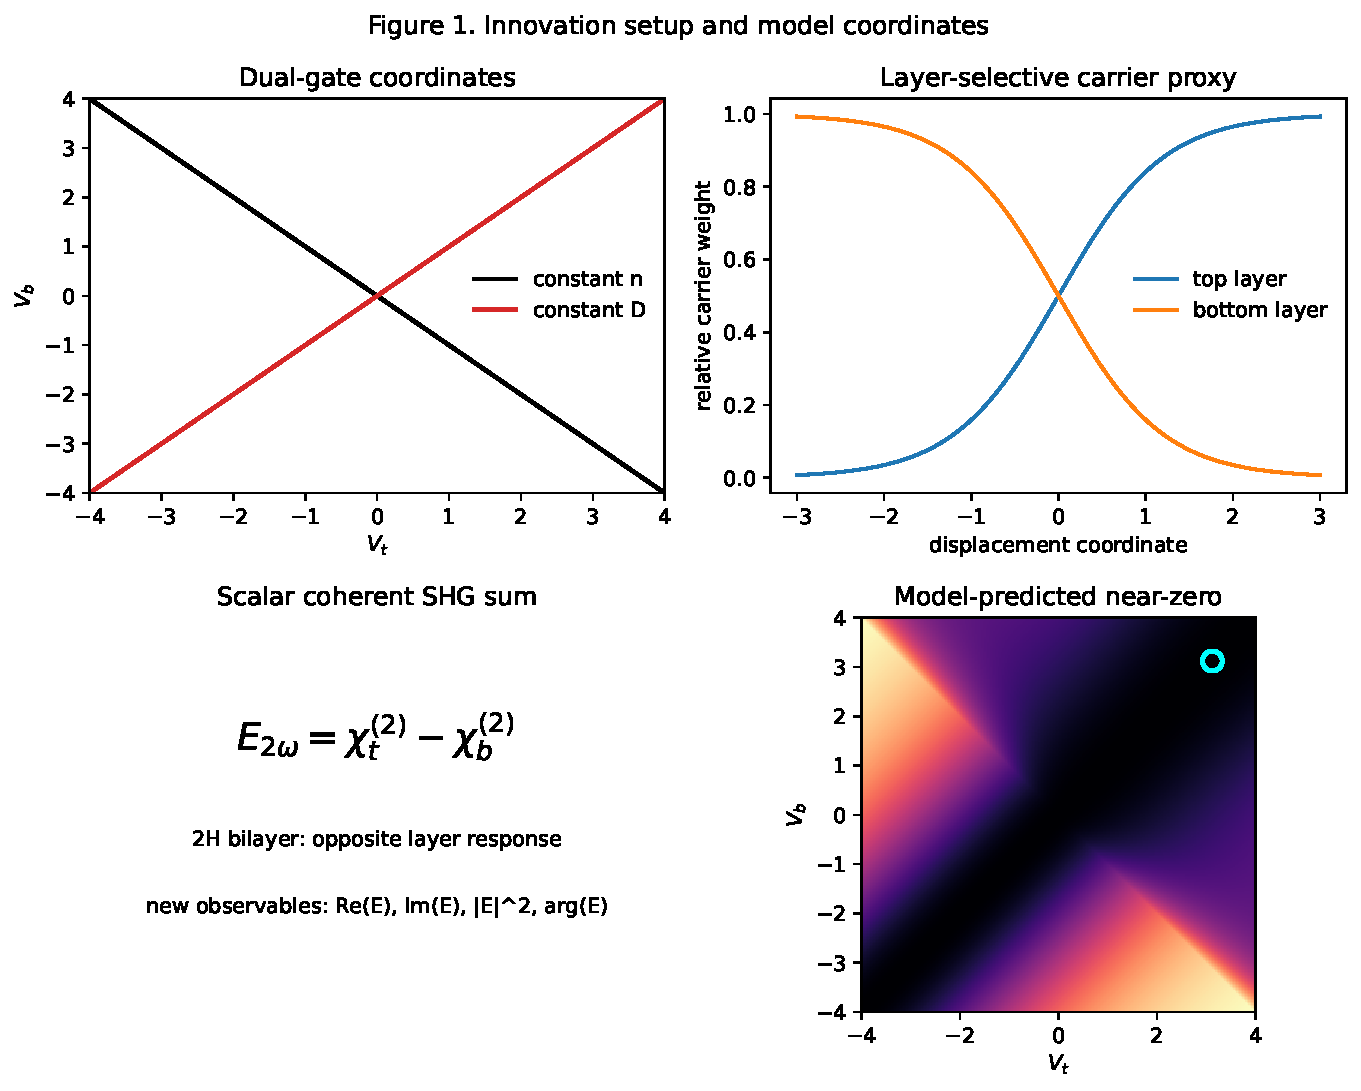
\includegraphics[width=\linewidth]{figure_1_setup_coordinates.pdf}
  \caption{创新机制起点和模型坐标。该图不是 Cha 2024 原图复现，而是说明本文如何从双栅、层选择性 exciton-polaron 和 2H 相干场求和出发，转向 $\mathrm{Re}(E)$、$\mathrm{Im}(E)$、$|E|^2$ 与 $\arg(E)$ 等复场观测量。}
\end{figure}

\begin{figure}[htbp]
  \centering
  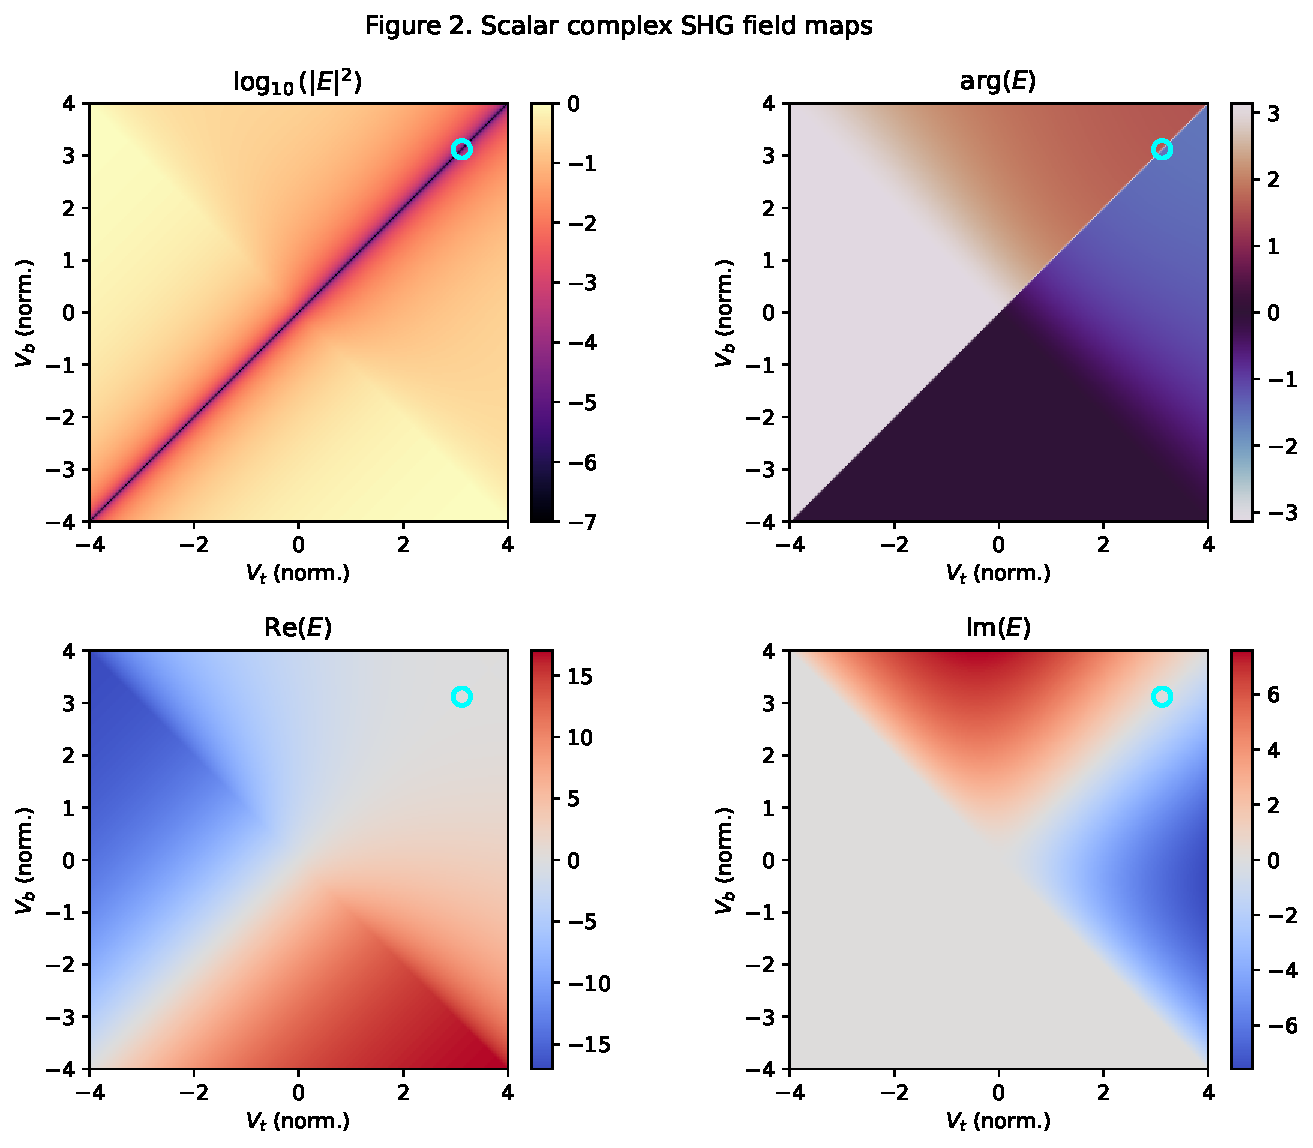
\includegraphics[width=\linewidth]{figure_2_complex_field_maps.pdf}
  \caption{标量复 SHG 场的多面板图：归一化强度、相位、实部和虚部。近零点附近强度出现暗点，同时相位发生快速变化；$\mathrm{Re}(E)$ 与 $\mathrm{Im}(E)$ 的过零结构共同定义了复场零点。}
\end{figure}

\begin{figure}[htbp]
  \centering
  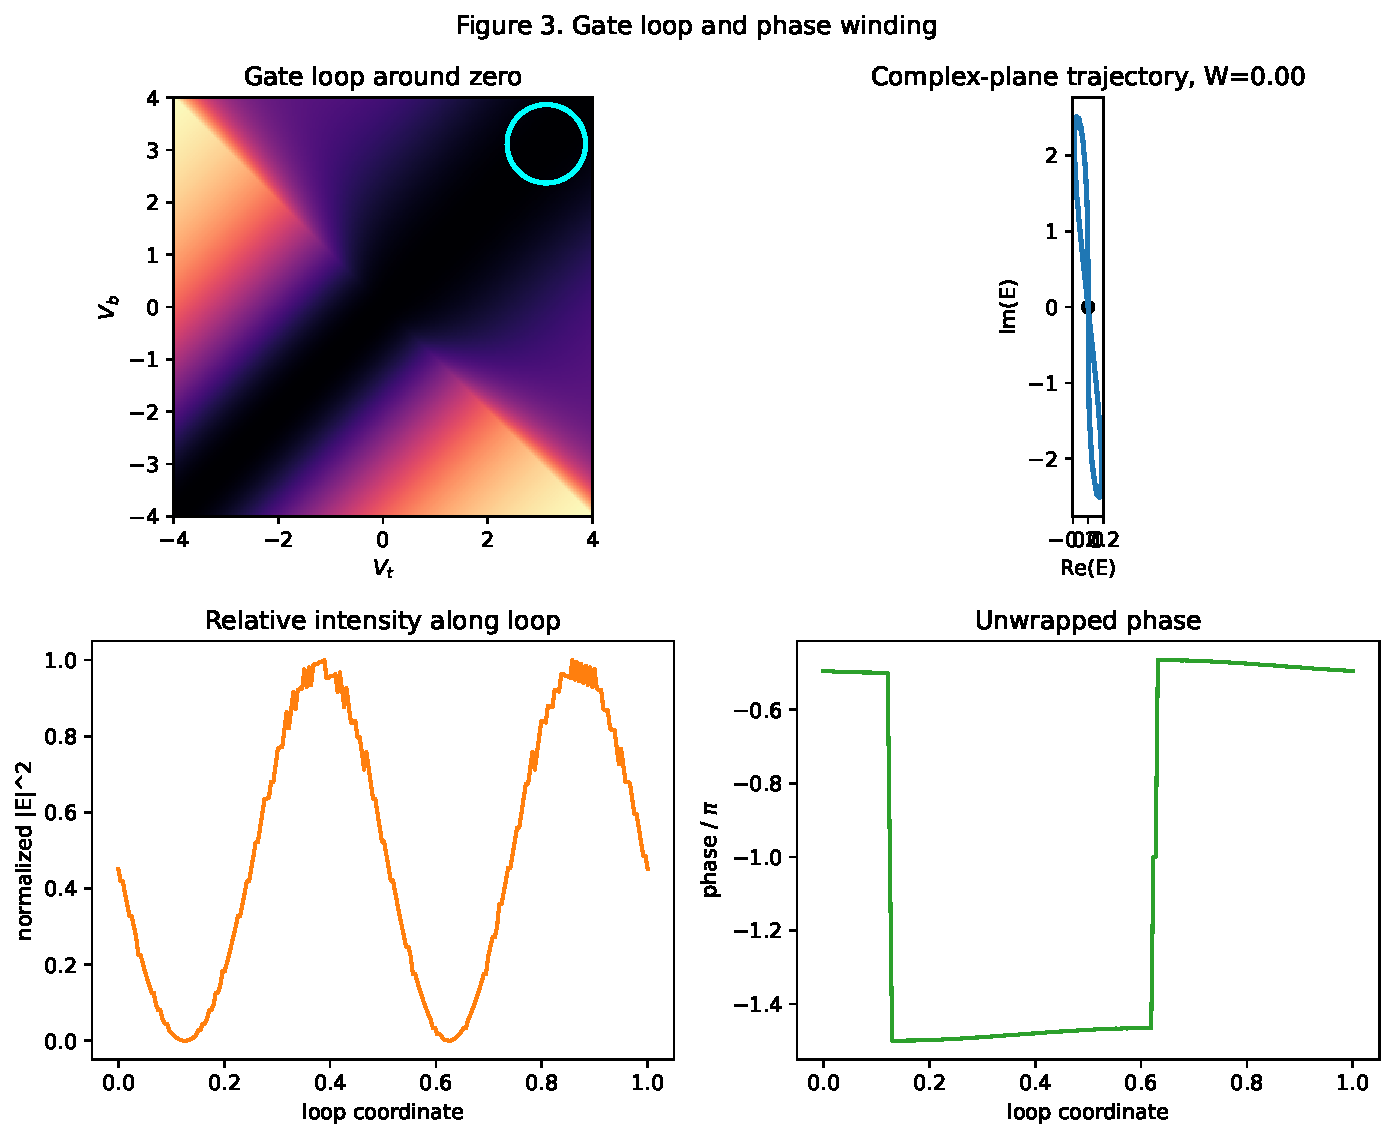
\includegraphics[width=\linewidth]{figure_3_gate_loop_winding.pdf}
  \caption{围绕近零点的闭合 gate loop，展示门压路径、复平面轨迹、路径上的相对强度和展开相位。复平面轨迹围绕原点时，相位沿路径累计变化接近 $2\pi$，形成数值认证的 phase winding。}
\end{figure}

\begin{figure}[htbp]
  \centering
  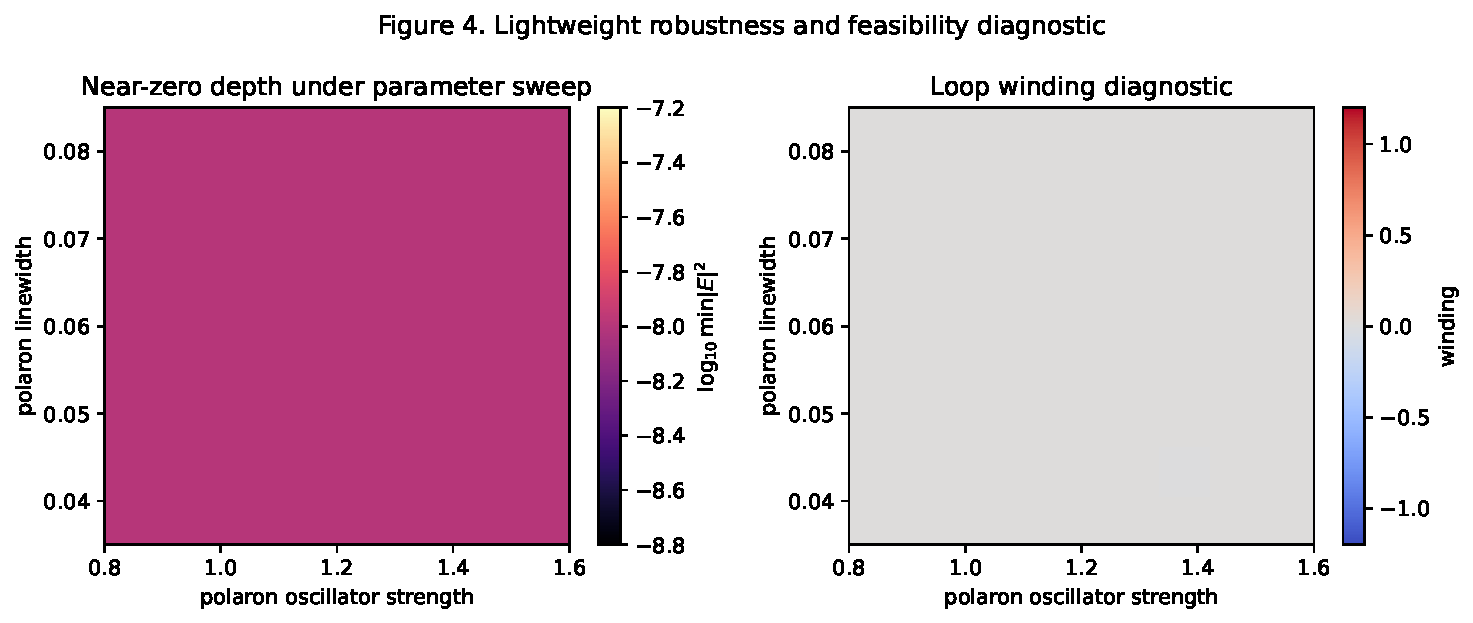
\includegraphics[width=\linewidth]{figure_4_robustness.pdf}
  \caption{轻量参数扫描检查现象是否依赖单点调参。通过改变 exciton-polaron 线宽和振子强度，可以观察近零点深度和 loop winding 的稳定区域。该图的目的不是完整优化，而是说明机制在一片合理参数区间内存在。}
\end{figure}

\begin{figure}[htbp]
  \centering
  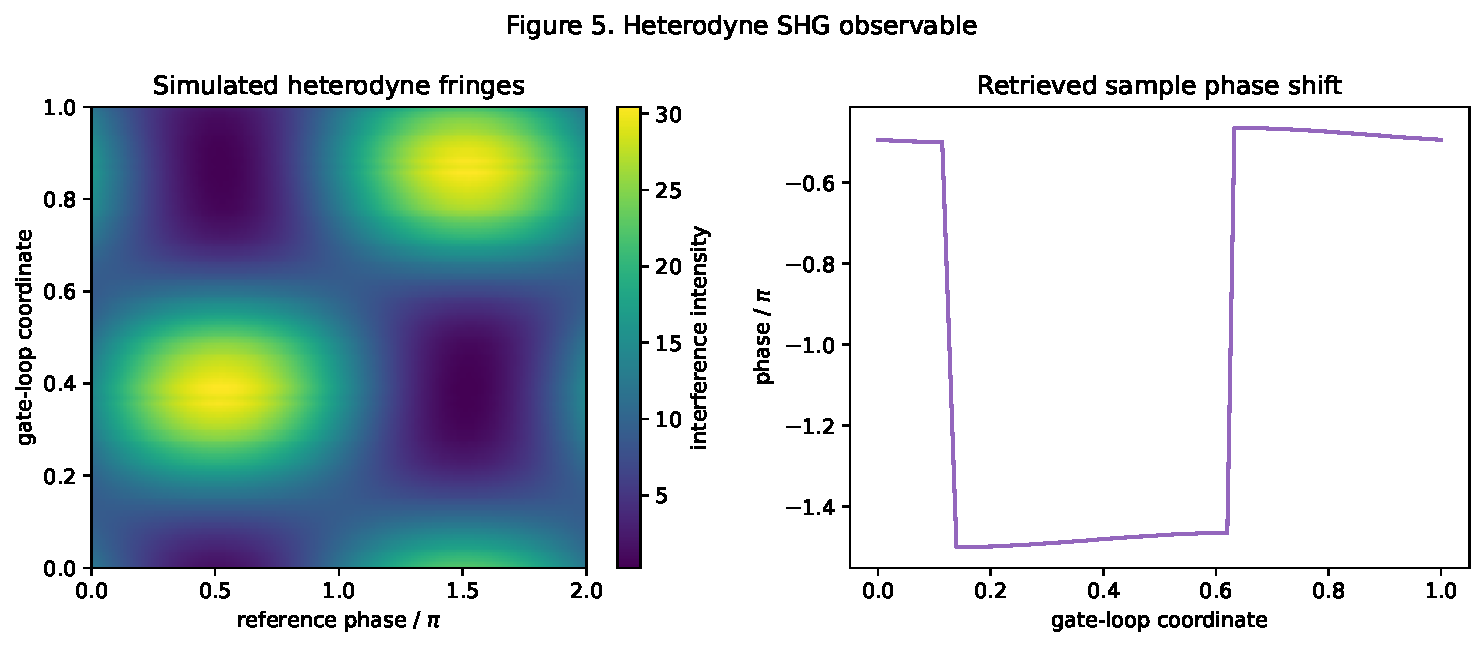
\includegraphics[width=\linewidth]{figure_5_heterodyne.pdf}
  \caption{将复场相位转换为 heterodyne SHG 可测量量。样品 SHG 与参考 SHG 干涉后，gate loop 上的相位变化表现为干涉条纹的整体平移和相位读出曲线的连续绕转。}
\end{figure}

\clearpage
\section{实验验证方案与对照}
实验上，主样品仍可采用 hBN-encapsulated 2H bilayer WSe$_2$ with graphite top and bottom gates。普通 SHG gate map 只能验证强度随门压变化，而本文真正需要的是 phase-resolved SHG 或 heterodyne SHG。样品 SHG 场与 quartz、BBO 或参考单层 WSe$_2$ 产生的参考 SHG 场干涉，通过扫描 reference phase 或 delay 恢复样品 $E_{2\omega}$ 的相位。

关键判据有四个。第一，沿特定 gate path 接近零点时 $|E_{2\omega}|^2$ 出现强度极小。第二，相同位置附近 $\mathrm{Re}(E_{2\omega})$ 与 $\mathrm{Im}(E_{2\omega})$ 同时接近零。第三，穿过零点附近时相位出现接近 $\pi$ 的跳变。第四，围绕零点闭合扫描时相位累计变化接近 $2\pi$。只有同时满足这些相位敏感判据，才能区分真正的相干零点和普通强度淬灭。

必要对照包括远离 exciton-polaron 共振的 pump detuning、monolayer WSe$_2$ 参考、以及 $D$ 反向时上下层角色交换导致零点位置镜像移动。远离共振后相位绕转应减弱或消失；单层样品缺少双层相干抵消通道；门压极性反转应改变层选择性极化子的空间分布。这些对照可以排除吸收、加热或普通 oscillator strength 变化导致的假零点解释。

\section{模型边界与可验证性}
\begin{itemize}[leftmargin=2em]
  \item 本文不拟合 Cha 2024 原始实验数据；Python 结果是创新机制的数值认证，而不是对实验图的复现。
  \item 本文不声称已经实验观测到 SHG zero 或 phase winding；实验部分是 proposed validation path。
  \item 本文不做 DFT、COMSOL 或 FDTD。核心问题是复 SHG 场的半经验相干机制，不是第一性原理材料参数提取或电磁场分布仿真。
  \item 本文不把 polarization singularity / Poincare sphere 作为 WSe$_2$ 主 claim。相关内容只作为 twisted heterobilayer 或偏振分辨扩展方向。
\end{itemize}

这些边界并不削弱本文的核心结论。相反，它们让本文的主张更明确：在已建立的双栅 exciton-polaron SHG 平台上，复数二次谐波场的零点和相位绕转是一个可以被数值认证、并可由 heterodyne SHG 直接检验的具体创新点。

\section{结论}
本文将主论文中的 layer-dependent exciton-polaron-enhanced SHG 从强度调制问题推进为标量复 SHG 场控制问题。通过 literature-constrained Python 模型，我们数值认证了双栅调控可以把 $E_{2\omega}$ 推近相干零点，并在闭合 gate loop 上产生相位绕转。这个结果给出了一个明确的创新路线：不是继续追求更大的 SHG enhancement，而是用双栅把 exciton-polaron 态变成可编程的非线性相位源。

\begin{thebibliography}{9}
\bibitem{cha2024}
S. Cha, T. Ouyang, T. Taniguchi, K. Watanabe, N. M. Gabor, and C. H. Lui, ``Enhancing Resonant Second-Harmonic Generation in Bilayer WSe2 by Layer-Dependent Exciton-Polaron Effect,'' \emph{Nano Letters} 24, 14847--14853 (2024). DOI: 10.1021/acs.nanolett.4c04544.

\bibitem{seyler2015}
K. L. Seyler et al., ``Electrical Control of Second-Harmonic Generation in a WSe2 Monolayer Transistor,'' \emph{Nature Nanotechnology} 10, 407--411 (2015). DOI: 10.1038/nnano.2015.73.

\bibitem{kim2020}
W. Kim, J. Y. Ahn, J. Oh, J. H. Shim, and S. Ryu, ``Second-Harmonic Young Interference in Atom-Thin Heterocrystals,'' \emph{Nano Letters} 20, 8825 (2020). DOI: 10.1021/acs.nanolett.0c03763.

\bibitem{wang2026}
Y. Wang et al., ``Destructive interference of second harmonic generation in AA stacked MoTe2/WSe2,'' arXiv:2605.21231 (2026).

\bibitem{shaarp2022}
R. Zu et al., ``Analytical and numerical modeling of optical second harmonic generation in anisotropic crystals using \#SHAARP package,'' \emph{npj Computational Materials} 8, 246 (2022). DOI: 10.1038/s41524-022-00930-4.
\end{thebibliography}

\end{document}

